\documentclass[12pt, a4paper]{article}
\usepackage[utf8]{inputenc}
\usepackage[margin=1in]{geometry}
\usepackage{amsmath, amsfonts, amssymb, amsthm}
\usepackage{xcolor}
\usepackage{enumitem}
\usepackage{tikz}
\usetikzlibrary{arrows.meta, positioning, matrix, decorations.pathreplacing}

\definecolor{primary}{RGB}{30, 60, 90}
\definecolor{accent}{RGB}{70, 100, 130}

\begin{document}

\begin{center}
    {\LARGE \textbf{\color{primary} Implementation of Canonical Form}} \\[0.5em]
    {\large \textit{Notes on Filippov's Constructive Proof of Jordan Canonical Form}}
\end{center}

\vspace{1em}

\section*{\color{primary} Motivation}
Filippov's proof of the canonical form of Jordan Form is constructive, based on mathematical induction. This naturally leads the reader to wonder if they can implement this method in Python.

\section*{\color{primary} Filippov's Method and Its Obstacles to Direct Python Code}

\begin{description}[font=\normalfont\bfseries\color{accent}, leftmargin=1.5em]
    \item[Step 1.] Find an eigenvalue $\lambda$ of input linear transform / matrix $T \longrightarrow$ use power iteration method to compute eigenvalue.
    \item[Step 2.] Let $A = T - \lambda I$. Define $\hat{T} = T\vert_{\text{range}(\mathcal{C}(A))}$.
    \item[Step 3.] Since $A$'s null space has at least one vector, aka the eigenvector belonging to $\lambda$, we know $\hat{T}$ is strictly less in dimension than $T$.
\end{description}

Thus by the hypothesis of mathematical induction:
\[
\hat{T} = \hat{M} \hat{J} \hat{M}^{-1}
\]
where $\hat{J}$ is of canonical Jordan form.

\vspace{0.5em}
More specifically, $\hat{J}$ is of the block-diagonal type:
\[
\hat{J} = \begin{pmatrix}
J_1 & & & & & \\
& J_2 & & & & \\
& & \ddots & & & \\
& & & J_t & & \\
& & & & Q_1 & \\
& & & & & \ddots & \\
& & & & & & Q_s
\end{pmatrix}
\]
where each $J_i$ ($i = 1 \dots t$) and $Q_j$ ($j = 1 \dots s$) are of Jordan block form. 

Put another way, under the domain $\mathcal{C}(A)$, $\hat{J}$ has $s + t$ eigenvectors, and each of them has a chain of eigenvectors. Here:
\begin{itemize}
    \item $J_i$ has the corresponding eigenvalue \textbf{not equal} to $\lambda$.
    \item $Q_j$ has eigenvalue \textbf{equal} to $\lambda$.
\end{itemize}

\vspace{1em}
Let us drill into one $Q_j$ block, say the dimension is $k_j$:
\[
Q_j = \begin{pmatrix}
\lambda & 1 & & \\
& \lambda & 1 & \\
& & \ddots & 1 \\
& & & \lambda
\end{pmatrix}
\]

\vspace{1em}
\noindent
\textbf{Basis Matrix Mapping for Block $Q_j$:}
\[
\hat{M} = \begin{pmatrix} \dots & \vec{m}_{Q_j, 1} & \vec{m}_{Q_j, 2} & \dots & \vec{m}_{Q_j, k_j} & \dots \end{pmatrix}
\]

\begin{center}
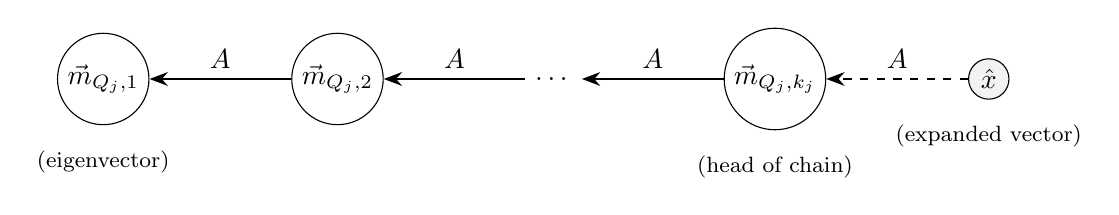
\begin{tikzpicture}[node distance=1.8cm, >=Stealth, auto]
    \node (v1) [draw, circle, inner sep=2pt] {$\vec{m}_{Q_j, 1}$};
    \node (v2) [draw, circle, inner sep=2pt, right=of v1] {$\vec{m}_{Q_j, 2}$};
    \node (dots) [right=of v2] {$\dots$};
    \node (vk) [draw, circle, inner sep=2pt, right=of dots] {$\vec{m}_{Q_j, k_j}$};
    \node (xhat) [draw, circle, inner sep=2pt, right=of vk, fill=gray!10] {$\hat{x}$};

    \draw[->, thick] (v2) -- node[above] {$A$} (v1);
    \draw[->, thick] (dots) -- node[above] {$A$} (v2);
    \draw[->, thick] (vk) -- node[above] {$A$} (dots);
    \draw[->, thick, dashed] (xhat) -- node[above] {$A$} (vk);
    
    \node[below=0.2cm of v1] {\footnotesize (eigenvector)};
    \node[below=0.2cm of vk] {\footnotesize (head of chain)};
    \node[below=0.2cm of xhat] {\footnotesize (expanded vector)};
\end{tikzpicture}
\end{center}

\vspace{1em}
\noindent
This is how the action of $A = T - \lambda I$ operates on the chain for $Q_j$:
\begin{align*}
    A \cdot \vec{m}_{Q_j, 1} &= 0 \\
    A \cdot \vec{m}_{Q_j, 2} &= \vec{m}_{Q_j, 1} \\
    &\;\;\vdots \\
    A \cdot \vec{m}_{Q_j, k_j} &= \vec{m}_{Q_j, k_j - 1}
\end{align*}

Note: $\vec{m}_{Q_j, 1}$ is eigenvector, $\vec{m}_{Q_j, k_j}$ is head of chain.

Here, due to the domain of $\hat{T}$ being $\mathcal{C}(A)$ (or $\text{range}(A)$), we know there exists a $\hat{x}$ such that:
\[
A\hat{x} = \vec{m}_{Q_j, k_j}
\]
Or, we can grow this chain by one.

\vspace{1em}
And for the $s$ $Q$-blocks, we also have $s$ eigenvectors like $\vec{m}_{Q_j, 1}$. Here, these vectors are all in the null space of $A$. We can expand them in the null space of $A$. The expanded vector corresponds to the new $Q$-blocks we added to $\hat{J}$ so that $\hat{J}$ can be expanded to $J$.

\vspace{2em}

\section*{\color{primary} Gaps Between Python Code Implementation}

The mathematical induction-based constructive proof by Filippov was introduced to me from the famous linear algebra book by Professor Strang from MIT. This proof should lead to a recursive function to generate canonical Jordan form if possible. (As in real numbers it may not always exist, but it always exists in complex numbers).

\begin{itemize}[leftmargin=1.5em]
    \item \textbf{Gap 1:} The first gap is about how to find $\hat{T}$ as a matrix. In code, we need a matrix representation of $\hat{T}$ in $\mathcal{C}(A)$ and pass it recursively to the CJM function itself.
    \item \textbf{Gap 2:} When expanding each $Q$ block / eigenvector chain, we need to solve $A\hat{x} = \vec{m}_{Q_j, k_j}$.
    \item \textbf{Gap 3:} For the $s$ eigenvectors in $Q$ blocks from $\hat{J}$, we need to expand these to the full null space of $A$, and use the newly added eigenvector to expand $\hat{J}$ to $J$.
    \item \textbf{Gap 4:} Find one eigenvalue $\lambda$ of matrix $T$. This is trickier than it looks by using the power iteration method.
\end{itemize}

\section*{\color{primary} How Do We Fill the Gap?}

\subsection*{\color{accent} 1. Find $\hat{T}$ Matrix}
A linear transformation is an abstract function mapping vectors from one space $\mathbb{R}^m$ to another space $\mathbb{R}^n$. Only when we fix a basis can we have a matrix.

So here, $\hat{T}$ should be calculated under a basis of its domain, a.k.a., $\mathcal{C}(A)$ or $\mathcal{C}(T - \lambda I)$.

So first, we need to find a basis. Here, any basis would do for our purpose, which is to pass $\hat{T}$ to the recursive function and get its Canonical Jordan Form $\hat{M}$ and $\hat{J}$. Thus, we can use either the Gram-Schmidt algorithm or RREF (Row Reduced Echelon Form). Let us get the basis as $\{\vec{p}_1, \vec{p}_2, \dots, \vec{p}_r\}$, where $r = \dim(\mathcal{C}(A))$, and $\vec{p}_i$ is represented in the standard basis $\{e\}$ given for $T$.

Then, as any linear transformation matrix under a certain basis does, we have the matrix representation of $\hat{T}$ in the $\{p\}$ basis as:
\[
\left( [\hat{T}\vec{p}_1]_{\{p\}}, [\hat{T}\vec{p}_2]_{\{p\}}, \dots, [\hat{T}\vec{p}_r]_{\{p\}} \right)
\]

Note that $\hat{T}\vec{p}_i$ is the vector $\vec{p}_i$'s image under $\hat{T}$ transformation in $\{p\}$ basis. Since the abstract vector $\vec{p}$ under $\hat{T}$ and $T$ has the same image abstract vector, we have:
\[
\hat{T}\vec{p}_{\{p\}} \longleftrightarrow T\vec{p}_{\{e\}}
\]

Using basis transformation for coordinates, we have:
\[
P \cdot \hat{T}\vec{p}_{\{p\}} = T\vec{p}_{\{e\}}, \quad \text{where } P = \begin{pmatrix} \vec{p}_1 & \vec{p}_2 & \dots & \vec{p}_r \end{pmatrix}_{\{e\}}
\]
Thus, we have:
\[
P \hat{T} = T P
\]
\[
\hat{T} = P^+ T P, \quad \text{where } P^+ \text{ is the left inverse of } P.
\]
As $P$'s column vectors are linearly independent, the left inverse exists:
\[
P^+ = (P^T P)^{-1} P^T
\]
So in summary:
\[
\hat{T} = (P^T P)^{-1} P^T T P
\]

\subsection*{\color{accent} 2. Solve $A\hat{x} = \vec{m}_{Q_j, k_j}$}
From $\hat{M}$ returned from the recursive call, we only have $\hat{m}_{Q_j, k_j}$ which lives in the $\{p\}$ basis. We first need to apply $\{p\}$ basis change to get $\vec{m}_{Q_j, k_j}$ in standard $\{e\}$ basis:
\[
\vec{m}_{Q_j, k_j} = P \hat{m}_{Q_j, k_j}
\]
Since $\vec{m}_{Q_j, k_j}$ lives in $\hat{T}$'s domain which is $\mathcal{C}(A)$, we know for sure $\vec{m}_{Q_j, k_j}$ is a linear combination of $\mathcal{C}(A)$ basis columns. Thus the above equation has a solution. We can put $(A \mid \vec{m}_{Q_j, k_j})$ as a matrix and perform RREF on it, verifying the last column does not contain a pivot point, as the condition there is a solution.

\subsection*{\color{accent} 3. Expand Null Space Basis}
Given $s$ eigenvectors from $Q_i$ ($i = 1 \dots s$), we need to expand them to the whole null space of $A$ and construct new $Q$-blocks to expand $\hat{J}$ to $J$.

Let us call the $s$ eigenvectors $\vec{v}_1, \vec{v}_2, \dots, \vec{v}_s$.

First, we can perform RREF on $A$ and get its basis for the null space of $A$ by setting free variables as $1$ and the rest as $0$ respectively. Then we will have $\vec{w}_1, \vec{w}_2, \dots, \vec{w}_{n-r}$ basis for $A$'s null space.

Then we perform another RREF in the following matrix constructed as:
\[
\begin{pmatrix} \vec{v}_1 & \vec{v}_2 & \dots & \vec{v}_s & \vec{w}_1 & \vec{w}_2 & \dots & \vec{w}_{n-r} \end{pmatrix}
\]
Since the first $s$ vectors are linearly independent, it would constitute the first $s$ pivot columns. The rest $n - r - s$ pivot columns correspond to the indices of vectors to be added in $\begin{pmatrix} \vec{v}_1 & \dots & \vec{v}_s & \vec{w}_1 & \dots & \vec{w}_{n-r} \end{pmatrix}$ matrix. Note, we pull the vectors from $\vec{w}_i$ ($i \in \{1 \dots n-r\}$), not the pivot columns from RREF.

\subsection*{\color{accent} 4. Power Iteration Method to Find Dominant Eigenvalue}
Power iteration method finds the dominant (largest absolute value) eigenvalue and eigenvector. This one has many pitfalls and is the major area to be improved.

The core idea of power method: given a random vector $\vec{v}$, it can be decomposed as a linear combination of eigenvectors:
\[
\vec{v} = c_1 \vec{w}_1 + c_2 \vec{w}_2 + \dots + c_n \vec{w}_n \quad \text{where } |c_1| \ge |c_2| \ge \dots \ge |c_n|
\]
If we keep applying $A$ to $\vec{v}$ and normalize it, we can let the direction of $\vec{w}_1$, aka largest eigenvalue's direction, dominate $A^k \vec{v}$. Thus we find $\vec{w}_1$ and $\lambda_1$. Mathematically, it is the following:
\begin{align*}
    \frac{A\vec{v}}{\|A\vec{v}\|} &= \frac{c_1 \lambda_1 \vec{w}_1 + c_2 \lambda_2 \vec{w}_2 + \dots + c_n \lambda_n \vec{w}_n}{\|A\vec{v}\|} \\[0.5em]
    \frac{A^2\vec{v}}{\|A^2\vec{v}\|} &= \frac{c_1 \lambda_1^2 \vec{w}_1 + c_2 \lambda_2^2 \vec{w}_2 + \dots + c_n \lambda_n^2 \vec{w}_n}{\|A^2\vec{v}\|} \\
    &\;\;\vdots \\
    \frac{A^n\vec{v}}{\|A^n\vec{v}\|} &= \frac{c_1 \vec{w}_1 + c_2 \left(\frac{\lambda_2}{\lambda_1}\right)^n \vec{w}_2 + \dots + c_n \left(\frac{\lambda_n}{\lambda_1}\right)^n \vec{w}_n}{\left\| c_1 \vec{w}_1 + c_2 \left(\frac{\lambda_2}{\lambda_1}\right)^n \vec{w}_2 + \dots + c_n \left(\frac{\lambda_n}{\lambda_1}\right)^n \vec{w}_n \right\|} \\[0.5em]
    &\approx \frac{c_1 \vec{w}_1}{\|c_1 \vec{w}_1\|}
\end{align*}

\subsubsection*{Pitfalls of Power Iteration}

\begin{enumerate}[label=\textbf{Pitfall \arabic*:}, leftmargin=1.5em]
    \item If largest $|\lambda_1| = |\lambda_2|$ and $\lambda_1 = -\lambda_2$, then this will not converge most likely. This issue we did not deal with and is an area to improve.
    \item If largest $\lambda_1$ is a complex number, we have $\bar{\lambda}_1$ also the largest. Then it will not converge just like Pitfall 1. In general, CJM form may not always be obtainable in real numbers. We may explore how to get CJM in complex numbers (which always exists) as a next step.
    \item If $\vec{v}$ is chosen happen to be orthogonal to $\vec{w}_1$, aka $c_1 = 0$, then we will miss this $\lambda$. We fix this by trying multiple random seeds $\vec{v}$.
    \item $\lambda = 0$ is also something we need to find in this case. Here, when we found eigenvector approximation $\frac{A^n\vec{v}}{\|A^n\vec{v}\|}$ as very close to $\vec{0}$ multiple times with different seed $\vec{v}$, we will check the input matrix is $[0]$ and return $\lambda$ as $0$.
\end{enumerate}

\vspace{2em}

\section*{\color{primary} RREF and Its Applications in Filippov's Proof of Jordan Form}

\subsection*{\color{accent} 1. What RREF Is and How It Works}

Row Reduced Echelon Form (RREF) is a form of a matrix that is reduced by two types of row operations (swapping rows, and adding a multiple of one row to another) until no more pivot points can be found. Performing row operations on a matrix $A$ to obtain its reduced form $R$ is equivalent to left-multiplying $A$ by invertible elementary matrices $P$ and $E$:

\[
\underbrace{P_k E_k \cdots P_1 E_1}_{T} A = R
\]

\[
A = T^{-1} R
\]

Here, $E$ represents row eliminations and $P$ represents row swaps. Because every elementary row operation is reversible, $E$ and $P$ possess inverses, which guarantees that $T$ also has an inverse $T^{-1}$.

\textbf{Pivot columns} are the columns in $R$ containing a pivot entry, while \textbf{free columns} are the non-pivot columns.

\[
\begin{pmatrix} \vec{a}_1 & \cdots & \vec{a}_3 & \cdots & \vec{a}_n \end{pmatrix}
\]
\[
\Big\downarrow \text{RREF}(A) \quad \Big\uparrow \text{corresponding to } A
\]
\[
\begin{pmatrix} \vec{v}_1 & \cdots & \vec{v}_3 & \cdots & \vec{v}_r \end{pmatrix}
\]

The pivot column indices identified in $R$, when mapped back to the original matrix $A$, specify $A$'s pivot columns.

\subsection*{\color{accent} 2. Why $A$'s Pivot Columns Form a Basis for Its Column Space $\mathcal{C}(A)$}

\subsubsection*{Linear Independence}
The pivot columns in $R$ are standard unit vectors—e.g., $\begin{pmatrix} 1 \\ 0 \\ 0 \end{pmatrix}, \begin{pmatrix} 0 \\ 1 \\ 0 \end{pmatrix}$—which are manifestly linearly independent. Let the pivot columns of $\text{RREF}(A)$ be denoted by $\vec{v}_1, \vec{v}_2, \dots, \vec{v}_r$.

Since $T A = R \iff A = T^{-1} R$, the corresponding original columns $\vec{a}_1, \vec{a}_2, \dots, \vec{a}_r$ of $A$ are also linearly independent. 

To prove this, suppose a linear combination equals zero:
\[
c_1 \vec{a}_1 + \cdots + c_r \vec{a}_r = \vec{0}
\]

Applying $T$ to both sides yields:
\[
c_1 (T \vec{a}_1) + \cdots + c_r (T \vec{a}_r) = \vec{0} \implies c_1 \vec{v}_1 + \cdots + c_r \vec{v}_r = \vec{0}
\]

Because $\vec{v}_1, \dots, \vec{v}_r$ are linearly independent, all coefficients must be zero ($c_1 = \cdots = c_r = 0$). Thus, $\vec{a}_1, \dots, \vec{a}_r$ are linearly independent.

\subsubsection*{Spanning the Column Space}
We know that $\mathcal{C}(A)$ has rank $r$, corresponding to the number of pivot positions. Having found $r$ linearly independent columns in $A$, they form a complete basis for $\mathcal{C}(A)$.

\subsection*{\color{accent} 3. The 3 Uses of RREF in Canonical Jordan Matrix (CJM)}

\subsubsection*{Use 1: Finding a Basis for the Range $\mathcal{C}(T - \lambda I)$}
RREF provides a systematic procedure to extract a maximal linearly independent subset of columns from $A$'s column space $\mathcal{C}(A)$. In Filippov's proof and CJM construction, we define $A = T - \lambda I$. Finding a basis for $\mathcal{C}(A)$ is directly implemented via the RREF algorithm.

\textbf{Why it works:} Row operations preserve linear dependency relationships among columns, allowing RREF to reliably identify pivot column indices.

\subsubsection*{Use 2: Growing Eigenvector Chains ($A\hat{x} = \vec{m}_{Q_j, k_j}$)}
For each Jordan block associated with eigenvalue $\lambda$, we take the top/last vector of the current chain, $\vec{m}_{Q_j, k_j}$, and solve $A\hat{x} = \vec{m}_{Q_j, k_j}$ to extend the chain by one step. We form the augmented matrix:
\[
\begin{pmatrix} \vec{a}_1 & \vec{a}_2 & \cdots & \vec{a}_r & \mid & \vec{m}_{Q_j, k_j} \end{pmatrix}
\]
and compute its RREF. 

\begin{itemize}
    \item \textbf{Consistency Check:} If the final column of the augmented matrix contains a pivot point, no solution exists because $\vec{m}_{Q_j, k_j} \notin \mathcal{C}(A)$. If the last column is free, the system is consistent and a solution exists.
    \item \textbf{Guarantee in Filippov's Proof:} In Filippov's proof, a solution is always guaranteed because $\hat{T}$ is defined strictly on the domain $\mathcal{C}(A)$. Since $\vec{m}_{Q_j, k_j} \in \mathcal{C}(A)$, the system $A\hat{x} = \vec{m}_{Q_j, k_j}$ is guaranteed to be consistent.
    \item \textbf{Meaning of Solution $\hat{x}$:} The solution vector $\hat{x}$ provides the exact scalar combination needed to express $\vec{m}_{Q_j, k_j}$ in terms of the columns of $A$.
\end{itemize}

\subsubsection*{Use 3: Expanding the Basis to the Null Space $\mathcal{N}(A)$}
The $s$ Jordan blocks in $\hat{J}$ corresponding to eigenvalue $\lambda$ yield $s$ independent eigenvectors residing in the null space $\mathcal{N}(A)$ where $A = T - \lambda I$. We must expand these $s$ vectors to form a complete basis for $\mathcal{N}(A)$, allowing us to extend $\hat{J}$ to $J$.

\textbf{Implementation Procedure:}
Given a set of $s$ linearly independent eigenvectors $(\vec{v}_1, \dots, \vec{v}_s)$ and a general basis $(\vec{w}_1, \dots, \vec{w}_r)$ for the space, we construct the matrix:
\[
\begin{pmatrix} \vec{v}_1 & \cdots & \vec{v}_s & \vec{w}_1 & \cdots & \vec{w}_r \end{pmatrix}
\]
and apply RREF:
\[
\Downarrow \text{RREF}
\]
\[
\text{Pivot Column Index Invariant}
\]

\textbf{Why it works:} RREF processes columns sequentially from left to right. Placing the existing eigenvectors $(\vec{v}_1, \dots, \vec{v}_s)$ first guarantees that RREF selects all $s$ of them as pivot columns. RREF then selects exactly $r - s$ additional vectors from $(\vec{w}_1, \dots, \vec{w}_r)$ corresponding to remaining pivot columns, completing the basis while discarding redundant vectors.

\end{document}
